\documentclass[10pt,twocolumn]{article}
\usepackage[margin=0.7in]{geometry}
\usepackage{booktabs,graphicx,amssymb}
\newcommand{\boxnote}{Box: interquartile range and median; whiskers: the most extreme replicate within 1.5 times the interquartile range; points: replicates beyond.}
\begin{document}
\begin{table*}[t]
\centering
\caption{RQ1: MAP per clone type (relevant = the query's clones of that type; the query's other same-functionality methods are removed from its ranking). Tree kernels on variant D at the settings tuned on separate queries. Mean = mean over the five types. Corpus: BigCloneBench true positives plus its 58,103 false positives (72,782 methods); false positives count as non-relevant, except exact copies of the query (ignored). 10 replicate query sets (seeds 55, 1375, 2084, 2802, 3389, 3501, 6251, 8241, 8828, 9080), each with 100 queries per clone type (T1, T2, VST3, ST3, MT3), drawn at random and independently of the other replicates; tuning queries excluded. Mean $\pm$ standard deviation over the 10 replicates. Best mean per column in bold. $^{+}$/$^{-}$: significantly better/worse than BM25; $^{\uparrow}$/$^{\downarrow}$: tree kernel significantly better/worse than fine-tuned CodeBERT. Significance: all distinct queries of the replicates pooled, paired bootstrap resampling functionalities, 95\%.}
\label{tab:rq1}
\footnotesize
\setlength{\tabcolsep}{3.5pt}
\begin{tabular}{llcccccc}
\toprule
Method & Setting & T1 & T2 & VST3 & ST3 & MT3 & Mean \\
\midrule
STK & $\lambda$=1.0 & \textbf{1.000}$\pm$0.000 & 0.994$\pm$0.003$^{+\uparrow}$ & 0.989$\pm$0.008$^{+\uparrow}$ & 0.911$\pm$0.017$^{+\uparrow}$ & 0.512$\pm$0.043 & 0.881$\pm$0.008$^{+\uparrow}$ \\
SSTK & $\lambda$=0.1 & \textbf{1.000}$\pm$0.000 & 0.994$\pm$0.003$^{+\uparrow}$ & \textbf{0.990}$\pm$0.005$^{+\uparrow}$ & 0.918$\pm$0.020$^{+\uparrow}$ & 0.520$\pm$0.045 & 0.885$\pm$0.009$^{+\uparrow}$ \\
PTK & $\lambda$=0.4, $\mu$=0.6 & \textbf{1.000}$\pm$0.000 & \textbf{0.994}$\pm$0.003$^{+\uparrow}$ & 0.987$\pm$0.008$^{+\uparrow}$ & \textbf{0.924}$\pm$0.019$^{+\uparrow}$ & \textbf{0.555}$\pm$0.044$^{+}$ & \textbf{0.892}$\pm$0.009$^{+\uparrow}$ \\
\midrule
BM25 & $k_1$=1.2, $b$=0.75 & 0.998$\pm$0.003 & 0.892$\pm$0.018 & 0.924$\pm$0.017 & 0.791$\pm$0.028 & 0.446$\pm$0.038 & 0.810$\pm$0.008 \\
CodeBERT zs & zero-shot & \textbf{1.000}$\pm$0.001 & 0.958$\pm$0.020$^{+}$ & 0.955$\pm$0.017 & 0.809$\pm$0.020 & 0.396$\pm$0.043 & 0.824$\pm$0.010 \\
CodeBERT ft & fine-tuned & \textbf{1.000}$\pm$0.001 & 0.931$\pm$0.018 & 0.949$\pm$0.020 & 0.780$\pm$0.020 & 0.461$\pm$0.035 & 0.824$\pm$0.009 \\
\bottomrule
\end{tabular}
\end{table*}

\begin{figure*}[t]\centering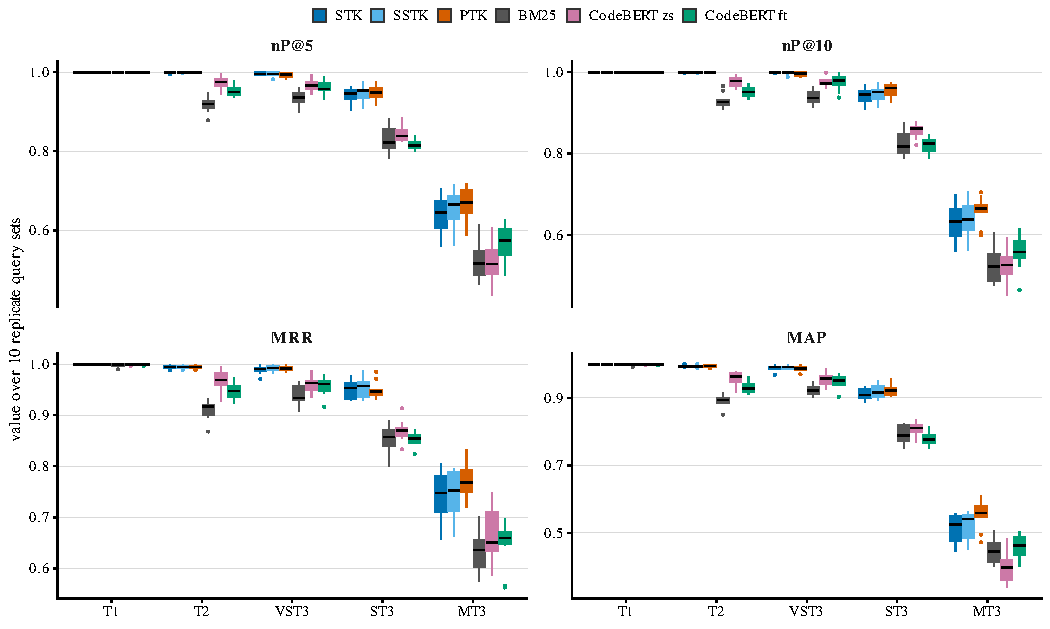
\includegraphics[width=\textwidth]{figures/rq1_metrics}\caption{RQ1 per clone type over 10 replicate query sets (100 queries per type each), corpus with false positives. \boxnote}\label{fig:rq1}\end{figure*}
\begin{table*}[t]
\centering
\caption{RQ1 and RQ2 under four metrics. RQ1: mean over the five clone types; RQ2: functional similarity (relevant = every method of the query's functionality, candidates = the whole corpus). nP@$k$ = relevant methods in the top $k$ divided by $\min(k, R)$, $R$ = the query's number of relevant methods; MRR = mean reciprocal rank of the first relevant method. Corpus: BigCloneBench true positives plus its 58,103 false positives (72,782 methods); false positives count as non-relevant, except exact copies of the query (ignored). 10 replicate query sets (seeds 55, 1375, 2084, 2802, 3389, 3501, 6251, 8241, 8828, 9080), each with 100 queries per clone type and 100 functional queries, drawn independently; tuning queries excluded. Mean $\pm$ standard deviation over the 10 replicates. Settings as in Table~\ref{tab:rq1}. Best mean per column in bold. $^{+}$/$^{-}$: significantly better/worse than BM25; $^{\uparrow}$/$^{\downarrow}$: tree kernel significantly better/worse than fine-tuned CodeBERT. Significance: all distinct queries of the replicates pooled, paired bootstrap resampling functionalities, 95\%.}
\label{tab:metrics}
\scriptsize
\setlength{\tabcolsep}{2pt}
\begin{tabular}{lcccccccc}
\toprule
 & \multicolumn{4}{c}{RQ1 (mean over the five types)} & \multicolumn{4}{c}{RQ2 (functional)} \\ \cmidrule(lr){2-5}\cmidrule(lr){6-9}
Method & nP@5 & nP@10 & MRR & MAP & nP@5 & nP@10 & MRR & MAP@R \\
\midrule
STK & 0.915$\pm$0.011$^{+\uparrow}$ & 0.914$\pm$0.011$^{+\uparrow}$ & 0.936$\pm$0.009$^{+\uparrow}$ & 0.881$\pm$0.008$^{+\uparrow}$ & 0.650$\pm$0.037$^{-\downarrow}$ & 0.599$\pm$0.036$^{-\downarrow}$ & 0.808$\pm$0.024$^{-\downarrow}$ & 0.137$\pm$0.021$^{-\downarrow}$ \\
SSTK & 0.919$\pm$0.011$^{+\uparrow}$ & 0.916$\pm$0.011$^{+\uparrow}$ & 0.937$\pm$0.010$^{+\uparrow}$ & 0.885$\pm$0.009$^{+\uparrow}$ & 0.652$\pm$0.032$^{-\downarrow}$ & 0.596$\pm$0.033$^{-\downarrow}$ & 0.810$\pm$0.021$^{-\downarrow}$ & 0.137$\pm$0.021$^{-\downarrow}$ \\
PTK & \textbf{0.921}$\pm$0.009$^{+\uparrow}$ & \textbf{0.922}$\pm$0.006$^{+\uparrow}$ & \textbf{0.941}$\pm$0.009$^{+\uparrow}$ & \textbf{0.892}$\pm$0.009$^{+\uparrow}$ & 0.611$\pm$0.039$^{-\downarrow}$ & 0.552$\pm$0.036$^{-\downarrow}$ & 0.774$\pm$0.034$^{-\downarrow}$ & 0.121$\pm$0.020$^{-\downarrow}$ \\
\midrule
BM25 & 0.841$\pm$0.008 & 0.845$\pm$0.009 & 0.866$\pm$0.008 & 0.810$\pm$0.008 & 0.751$\pm$0.028 & 0.708$\pm$0.023 & \textbf{0.879}$\pm$0.020 & 0.305$\pm$0.023 \\
CodeBERT zs & 0.860$\pm$0.012 & 0.866$\pm$0.009 & 0.893$\pm$0.011$^{+}$ & 0.824$\pm$0.010 & 0.628$\pm$0.021$^{-}$ & 0.573$\pm$0.021$^{-}$ & 0.797$\pm$0.019$^{-}$ & 0.109$\pm$0.015$^{-}$ \\
CodeBERT ft & 0.859$\pm$0.011 & 0.861$\pm$0.011 & 0.880$\pm$0.011 & 0.824$\pm$0.009 & \textbf{0.757}$\pm$0.032 & \textbf{0.728}$\pm$0.030 & 0.875$\pm$0.025 & \textbf{0.310}$\pm$0.025 \\
\bottomrule
\end{tabular}
\end{table*}

\begin{figure}[t]\centering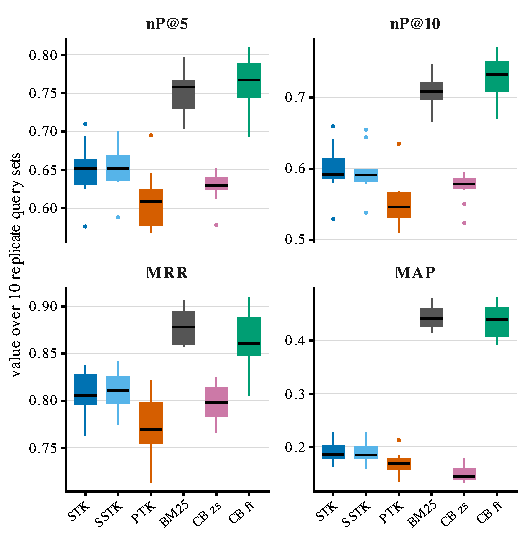
\includegraphics[width=\columnwidth]{figures/rq2_metrics}\caption{RQ2: functional similarity over 10 replicate query sets (100 queries each), corpus with false positives. \boxnote}\label{fig:rq2}\end{figure}
\begin{table*}[t]
\centering
\caption{RQ4: fusion of a tree kernel (variant D, tuned) with BM25 or with fine-tuned CodeBERT. Weighted sum = $W\cdot$TK + $(1-W)\cdot$other/max, $W$ tuned on the tuning queries for the RQ's measure; RRF = reciprocal rank fusion ($k$=60). The RQ1 fusions use PTK, the best kernel on RQ1; the RQ2 fusions use STK. Corpus: BigCloneBench true positives plus its 58,103 false positives (72,782 methods); false positives count as non-relevant, except exact copies of the query (ignored). 10 replicate query sets (seeds 55, 1375, 2084, 2802, 3389, 3501, 6251, 8241, 8828, 9080), each with 100 queries per clone type and 100 functional queries, drawn independently; tuning queries excluded. Mean $\pm$ standard deviation over the 10 replicates. Best mean per block and column in bold. $^{\dagger}$: significantly better than both components. Significance: all distinct queries of the replicates pooled, paired bootstrap resampling functionalities, 95\%.}
\label{tab:rq4}
\footnotesize
\setlength{\tabcolsep}{3.5pt}
\begin{tabular}{lcccc}
\toprule
 & \multicolumn{3}{c}{RQ1 (MAP)} & RQ2 \\ \cmidrule(lr){2-4} \cmidrule(lr){5-5}
Method & ST3 & MT3 & Mean & MAP@R \\
\midrule
\multicolumn{5}{l}{\emph{PTK + BM25, $W$ tuned for RQ1}} \\
\quad PTK & 0.924$\pm$0.019 & 0.555$\pm$0.044 & 0.892$\pm$0.009 & -- \\
\quad BM25 & 0.791$\pm$0.028 & 0.446$\pm$0.038 & 0.810$\pm$0.008 & -- \\
\quad Weighted sum ($W$=0.9) & \textbf{0.943}$\pm$0.017$^{\dagger}$ & \textbf{0.661}$\pm$0.043$^{\dagger}$ & \textbf{0.918}$\pm$0.008$^{\dagger}$ & -- \\
\quad RRF & 0.911$\pm$0.018 & 0.600$\pm$0.033 & 0.896$\pm$0.006 & -- \\
\midrule
\multicolumn{5}{l}{\emph{PTK + CodeBERT ft, $W$ tuned for RQ1}} \\
\quad PTK & 0.924$\pm$0.019 & 0.555$\pm$0.044 & 0.892$\pm$0.009 & -- \\
\quad CodeBERT ft & 0.780$\pm$0.020 & 0.461$\pm$0.035 & 0.824$\pm$0.009 & -- \\
\quad Weighted sum ($W$=0.6) & \textbf{0.944}$\pm$0.013$^{\dagger}$ & \textbf{0.672}$\pm$0.039$^{\dagger}$ & \textbf{0.920}$\pm$0.007$^{\dagger}$ & -- \\
\quad RRF & 0.909$\pm$0.013 & 0.619$\pm$0.037$^{\dagger}$ & 0.898$\pm$0.008 & -- \\
\midrule
\multicolumn{5}{l}{\emph{STK + BM25, $W$ tuned for RQ2}} \\
\quad STK & -- & -- & -- & 0.137$\pm$0.021 \\
\quad BM25 & -- & -- & -- & \textbf{0.305}$\pm$0.023 \\
\quad Weighted sum ($W$=0.0) & -- & -- & -- & \textbf{0.305}$\pm$0.023 \\
\quad RRF & -- & -- & -- & 0.229$\pm$0.021 \\
\midrule
\multicolumn{5}{l}{\emph{STK + CodeBERT ft, $W$ tuned for RQ2}} \\
\quad STK & -- & -- & -- & 0.137$\pm$0.021 \\
\quad CodeBERT ft & -- & -- & -- & 0.310$\pm$0.025 \\
\quad Weighted sum ($W$=0.2) & -- & -- & -- & \textbf{0.320}$\pm$0.026$^{\dagger}$ \\
\quad RRF & -- & -- & -- & 0.245$\pm$0.020 \\
\bottomrule
\end{tabular}
\end{table*}

\begin{figure*}[t]\centering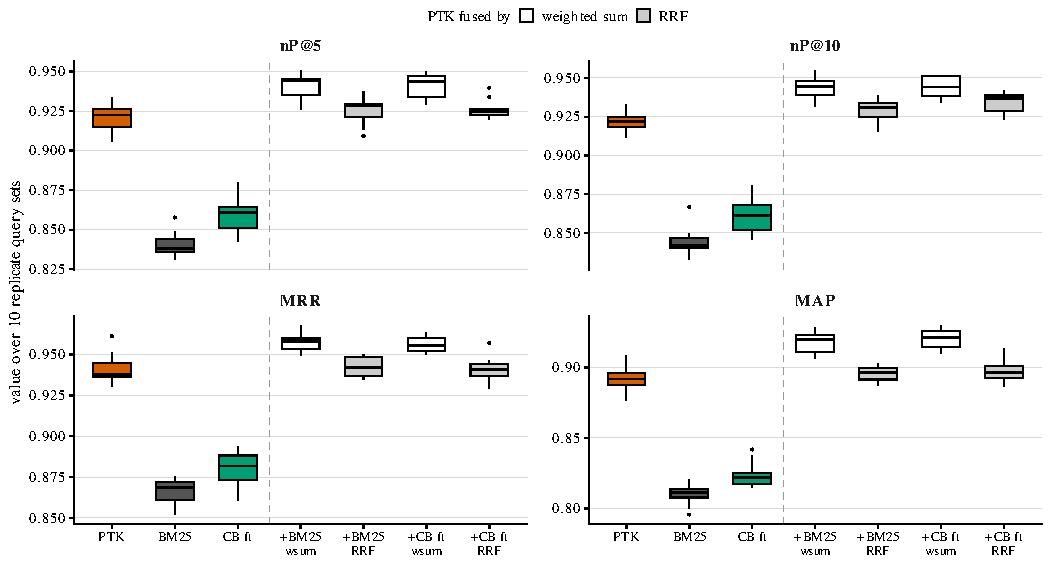
\includegraphics[width=\textwidth]{figures/rq4_fusion_rq1}\caption{RQ4, syntactic clones: PTK, BM25, fine-tuned CodeBERT and the fusions of PTK with each (weighted sum at the tuned $W$; RRF); mean over the five clone types, 10 replicate query sets. \boxnote}\label{fig:rq4a}\end{figure*}
\begin{figure*}[t]\centering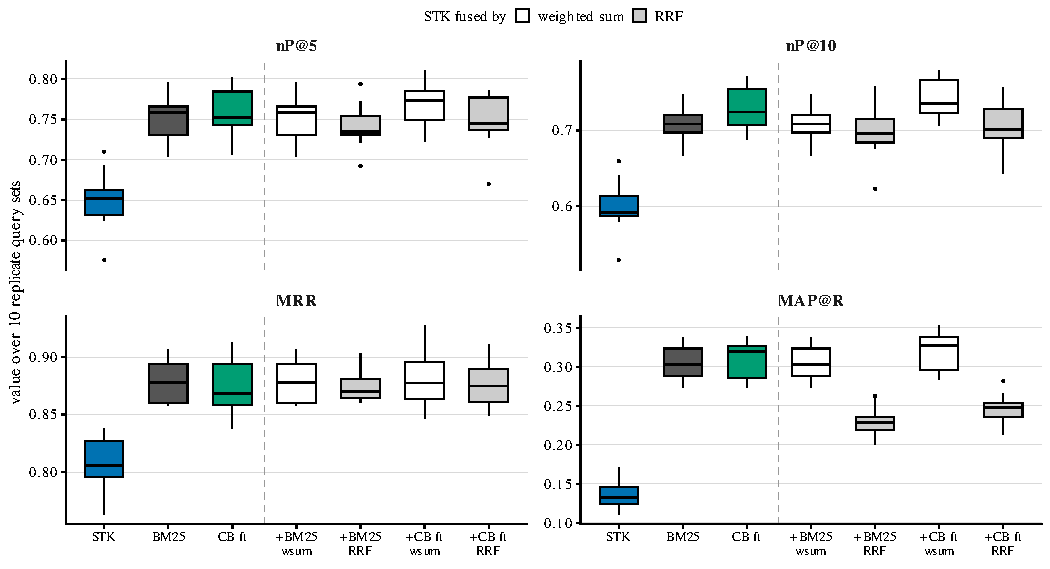
\includegraphics[width=\textwidth]{figures/rq4_fusion_rq2}\caption{RQ4, functional similarity: STK, BM25, fine-tuned CodeBERT and the fusions of STK with each; 10 replicate query sets. \boxnote}\label{fig:rq4b}\end{figure*}
\begin{table*}[t]
\centering
\caption{Size and complexity: RQ1 (MAP, mean over the five clone types) and RQ2 (functional MAP@R) per group of the query. Groups of the query: small = at most 6 lines of code (physical lines of the method), large = at least 10; low = McCabe cyclomatic complexity at most 10, high = above 10 (Checkstyle 10.21.1, default counting). Corpus: BigCloneBench true positives plus its 58,103 false positives (72,782 methods); false positives count as non-relevant, except exact copies of the query (ignored); candidates are not restricted by group. Per seed (10 seeds, those of the replicate query sets), group and query set, 100 queries at random from the group, or the whole group when it has fewer (small T2: 53, small VST3: 12, high T2: 57 queries). Tree kernels on variant D at the tuned settings. Mean $\pm$ standard deviation over the 10 seeds; best mean per column in bold. Last row: distinct queries over all seeds (functionalities). Table~\ref{tab:sizecxint} tests whether the differences between methods change between groups.}
\label{tab:sizecx}
\scriptsize
\setlength{\tabcolsep}{3pt}
\begin{tabular}{lcccccccc}
\toprule
 & \multicolumn{4}{c}{RQ1: MAP (mean over the five types)} & \multicolumn{4}{c}{RQ2: MAP@R} \\ \cmidrule(lr){2-5}\cmidrule(lr){6-9}
 & \multicolumn{2}{c}{Size} & \multicolumn{2}{c}{Complexity} & \multicolumn{2}{c}{Size} & \multicolumn{2}{c}{Complexity} \\ \cmidrule(lr){2-3}\cmidrule(lr){4-5}\cmidrule(lr){6-7}\cmidrule(lr){8-9}
Method & small & large & low & high & small & large & low & high \\
\midrule
STK & 0.875$\pm$0.006 & 0.868$\pm$0.006 & 0.873$\pm$0.009 & 0.935$\pm$0.005 & 0.503$\pm$0.024 & 0.092$\pm$0.013 & 0.134$\pm$0.019 & 0.041$\pm$0.007 \\
SSTK & 0.885$\pm$0.006 & 0.872$\pm$0.005 & 0.877$\pm$0.007 & 0.935$\pm$0.005 & 0.505$\pm$0.025 & 0.092$\pm$0.014 & 0.134$\pm$0.019 & 0.041$\pm$0.007 \\
PTK & \textbf{0.913}$\pm$0.008 & \textbf{0.874}$\pm$0.009 & \textbf{0.893}$\pm$0.006 & 0.828$\pm$0.008 & 0.488$\pm$0.030 & 0.082$\pm$0.016 & 0.122$\pm$0.020 & 0.036$\pm$0.006 \\
\midrule
BM25 & 0.631$\pm$0.006 & 0.826$\pm$0.010 & 0.803$\pm$0.009 & \textbf{0.961}$\pm$0.005 & \textbf{0.605}$\pm$0.020 & 0.274$\pm$0.031 & 0.315$\pm$0.025 & \textbf{0.171}$\pm$0.019 \\
CodeBERT zs & 0.821$\pm$0.006 & 0.816$\pm$0.010 & 0.816$\pm$0.010 & 0.904$\pm$0.009 & 0.434$\pm$0.031 & 0.072$\pm$0.009 & 0.104$\pm$0.016 & 0.043$\pm$0.008 \\
CodeBERT ft & 0.699$\pm$0.006 & 0.822$\pm$0.012 & 0.819$\pm$0.009 & 0.909$\pm$0.010 & 0.586$\pm$0.021 & \textbf{0.279}$\pm$0.026 & \textbf{0.318}$\pm$0.027 & 0.169$\pm$0.021 \\
\midrule
Queries & 1,425 (22) & 4,025 (38) & 4,135 (40) & 1,422 (26) & 593 (28) & 957 (37) & 965 (41) & 802 (31) \\
\bottomrule
\end{tabular}
\end{table*}

\begin{table*}[!htbp]
\centering
\caption{RQ3, size and complexity: does the difference between two methods change between groups? Each cell is $D = (A - B)_{1} - (A - B)_{2}$, the difference between methods $A$ and $B$ on the first group minus that on the second, with its 95\% confidence interval in the row below; positive: $A$'s advantage is larger (or its disadvantage smaller) on the first group. Bold: the interval excludes 0. All distinct queries of the seeds pooled; paired bootstrap resampling functionalities jointly for both groups (2,000 resamples). RQ1: mean over the five clone types; RQ2: functional similarity. \emph{Large only}: complexity compared among queries with at least 10 lines (every high-complexity query is large). Groups and setup as in Table~\ref{tab:sizecx}.}
\label{tab:sizecxint}
\scriptsize
\setlength{\tabcolsep}{3pt}
\begin{tabular}{lcccccc}
\toprule
 & \multicolumn{3}{c}{RQ1: MAP (mean over the five types)} & \multicolumn{3}{c}{RQ2: MAP (functional)} \\ \cmidrule(lr){2-4}\cmidrule(lr){5-7}
$A - B$ & small $-$ large & low $-$ high & low $-$ high & small $-$ large & low $-$ high & low $-$ high \\
 &  &  & (large only) &  &  & (large only) \\
\midrule
\quad PTK $-$ BM25 & \textbf{+0.235} & \textbf{+0.223} & \textbf{+0.191} & +0.099 & -0.070 & -0.077 \\
 & [+0.086, +0.388] & [+0.174, +0.264] & [+0.148, +0.226] & [-0.123, +0.265] & [-0.134, +0.014] & [-0.145, +0.009] \\[2pt]
\quad PTK $-$ CB ft & +0.103 & \textbf{+0.138} & \textbf{+0.136} & +0.123 & -0.061 & \textbf{-0.068} \\
 & [-0.008, +0.201] & [+0.086, +0.193] & [+0.084, +0.188] & [-0.016, +0.237] & [-0.126, +0.001] & [-0.138, -0.005] \\[2pt]
\quad STK $-$ BM25 & \textbf{+0.202} & \textbf{+0.097} & \textbf{+0.068} & +0.122 & -0.059 & -0.068 \\
 & [+0.052, +0.361] & [+0.051, +0.131] & [+0.027, +0.097] & [-0.047, +0.264] & [-0.117, +0.014] & [-0.132, +0.004] \\[2pt]
\quad STK $-$ CB ft & +0.070 & +0.012 & +0.012 & \textbf{+0.146} & -0.050 & \textbf{-0.058} \\
 & [-0.042, +0.180] & [-0.029, +0.052] & [-0.027, +0.048] & [+0.051, +0.240] & [-0.111, +0.006] & [-0.122, -0.002] \\[2pt]
\quad SSTK $-$ BM25 & \textbf{+0.208} & \textbf{+0.101} & \textbf{+0.071} & +0.120 & -0.060 & -0.069 \\
 & [+0.056, +0.361] & [+0.054, +0.135] & [+0.030, +0.101] & [-0.052, +0.263] & [-0.118, +0.011] & [-0.132, +0.003] \\[2pt]
\quad SSTK $-$ CB ft & +0.076 & +0.015 & +0.015 & \textbf{+0.144} & -0.051 & \textbf{-0.059} \\
 & [-0.041, +0.180] & [-0.024, +0.057] & [-0.024, +0.053] & [+0.048, +0.238] & [-0.112, +0.005] & [-0.123, -0.003] \\[2pt]
\cmidrule(lr){1-7}
\quad CB ft $-$ BM25 & \textbf{+0.132} & \textbf{+0.085} & \textbf{+0.056} & -0.024 & -0.009 & -0.009 \\
 & [+0.026, +0.227] & [+0.021, +0.142] & [+0.001, +0.106] & [-0.134, +0.048] & [-0.049, +0.050] & [-0.050, +0.048] \\[2pt]
\bottomrule
\end{tabular}
\end{table*}

\begin{figure*}[t]\centering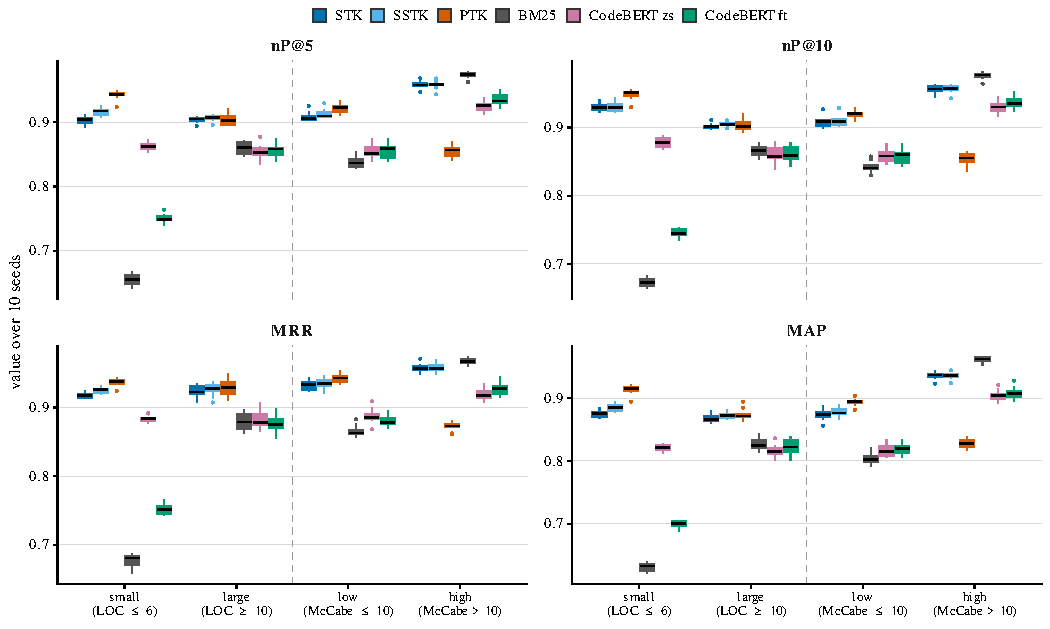
\includegraphics[width=\textwidth]{figures/size_complexity_rq1}\caption{Size and complexity, RQ1: mean over the five clone types per group of the query, 10 seeds (groups as in Table~\ref{tab:sizecx}). \boxnote}\label{fig:sizecx1}\end{figure*}
\begin{figure*}[t]\centering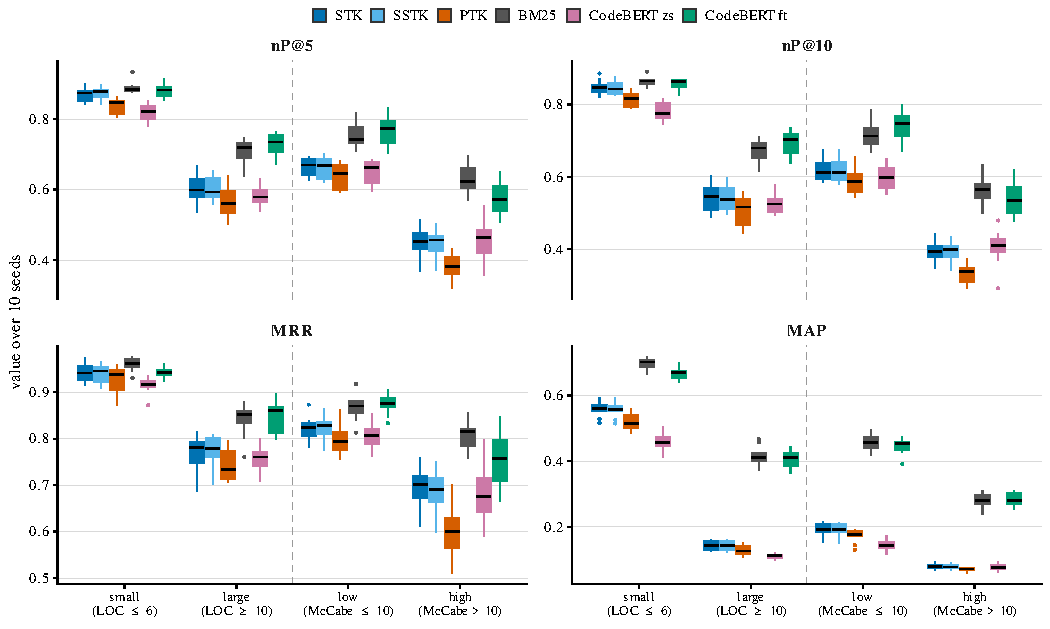
\includegraphics[width=\textwidth]{figures/size_complexity_rq2}\caption{Size and complexity, RQ2: functional similarity per group of the query, 10 seeds. \boxnote}\label{fig:sizecx2}\end{figure*}
\begin{table*}[!htbp]
\centering
\caption{RQ4, hybrid on every eligible query (T1 3,746, T2 998, VST3 1,991, ST3 4,652, MT3 7,722, functional 14,587). Corpus: BigCloneBench true positives plus its 58,103 false positives (72,782 methods); false positives count as non-relevant, except exact copies of the query (ignored). Hybrid: BM25's top $k$ ($k$ = 100, 200, not tuned) re-ranked by the tree kernel (variant D, tuned settings); below rank $k$ the BM25 order is kept. Each cell: value over all queries, 95\% confidence interval below (bootstrap resampling functionalities). RQ1: per clone type and Mean over the five types; RQ2: functional similarity. Best value per column in bold. $^{+}$/$^{-}$: significantly better/worse than BM25; $^{\uparrow}$/$^{\downarrow}$: significantly better/worse than fine-tuned CodeBERT (paired bootstrap over functionalities, 95\%). Full-ranking tree kernels were run on the replicate query sets only (Table~\ref{tab:hybridrep}).}
\label{tab:hybridfull}
\scriptsize
\setlength{\tabcolsep}{3pt}
\begin{tabular}{lccccccc}
\toprule
 & \multicolumn{6}{c}{RQ1: MAP} & RQ2: MAP \\ \cmidrule(lr){2-7}\cmidrule(lr){8-8}
Method & T1 & T2 & VST3 & ST3 & MT3 & Mean & functional \\
\midrule
\quad BM25 & 0.999 & 0.886 & 0.934 & 0.771 & 0.453 & 0.808 & \textbf{0.443} \\
 & [0.997, 1.000] & [0.852, 0.936] & [0.902, 0.972] & [0.705, 0.845] & [0.400, 0.533] & [0.781, 0.850] & [0.363, 0.544] \\[2pt]
\quad CodeBERT zs & 0.999 & 0.970 & 0.959 & 0.794 & 0.392 & 0.823 & 0.144 \\
 & [0.997, 1.000] & [0.960, 0.986] & [0.944, 0.977] & [0.747, 0.866] & [0.339, 0.485] & [0.803, 0.859] & [0.111, 0.196] \\[2pt]
\quad CodeBERT ft & \textbf{1.000} & 0.937 & 0.942 & 0.767 & 0.461 & 0.821 & 0.421 \\
 & [0.999, 1.000] & [0.877, 0.978] & [0.904, 0.970] & [0.688, 0.857] & [0.384, 0.578] & [0.775, 0.875] & [0.345, 0.520] \\[2pt]
\cmidrule(lr){1-8}
\quad BM25$\rightarrow$STK ($k$=100) & \textbf{1.000} & 0.944$^{+}$ & 0.951$^{+}$ & 0.814$^{+}$ & 0.478$^{+}$ & 0.837$^{+}$ & 0.440$^{-}$ \\
 & [1.000, 1.000] & [0.913, 0.986] & [0.924, 0.982] & [0.757, 0.882] & [0.426, 0.560] & [0.814, 0.876] & [0.360, 0.541] \\[2pt]
\quad BM25$\rightarrow$STK ($k$=200) & \textbf{1.000} & \textbf{0.976}$^{+}$ & 0.960$^{+}$ & 0.840$^{+\uparrow}$ & 0.494$^{+}$ & 0.854$^{+}$ & 0.437$^{-}$ \\
 & [1.000, 1.000] & [0.967, 0.990] & [0.940, 0.988] & [0.788, 0.902] & [0.440, 0.580] & [0.833, 0.887] & [0.357, 0.535] \\[2pt]
\quad BM25$\rightarrow$SSTK ($k$=100) & \textbf{1.000} & 0.944$^{+}$ & 0.952$^{+}$ & 0.815$^{+}$ & 0.479$^{+}$ & 0.838$^{+}$ & 0.440$^{-}$ \\
 & [1.000, 1.000] & [0.913, 0.986] & [0.924, 0.982] & [0.759, 0.880] & [0.427, 0.561] & [0.814, 0.877] & [0.360, 0.541] \\[2pt]
\quad BM25$\rightarrow$SSTK ($k$=200) & \textbf{1.000} & \textbf{0.976}$^{+}$ & \textbf{0.961}$^{+}$ & \textbf{0.842}$^{+\uparrow}$ & 0.496$^{+}$ & 0.855$^{+}$ & 0.436$^{-}$ \\
 & [1.000, 1.000] & [0.967, 0.990] & [0.940, 0.988] & [0.792, 0.901] & [0.442, 0.582] & [0.834, 0.887] & [0.357, 0.535] \\[2pt]
\quad BM25$\rightarrow$PTK ($k$=100) & \textbf{1.000} & 0.944$^{+}$ & 0.951$^{+}$ & 0.811$^{+}$ & 0.482$^{+}$ & 0.838$^{+}$ & 0.442 \\
 & [1.000, 1.000] & [0.913, 0.986] & [0.924, 0.982] & [0.759, 0.875] & [0.431, 0.568] & [0.814, 0.876] & [0.361, 0.543] \\[2pt]
\quad BM25$\rightarrow$PTK ($k$=200) & \textbf{1.000} & \textbf{0.976}$^{+}$ & 0.960$^{+}$ & 0.838$^{+}$ & \textbf{0.508}$^{+}$ & \textbf{0.857}$^{+}$ & 0.441 \\
 & [1.000, 1.000] & [0.967, 0.990] & [0.939, 0.988] & [0.793, 0.893] & [0.454, 0.597] & [0.837, 0.888] & [0.360, 0.540] \\[2pt]
\bottomrule
\end{tabular}
\end{table*}

\begin{table*}[t]
\centering
\caption{Hybrid against the full-ranking tree kernels on the 10 replicate query sets (each with 100 queries per clone type for RQ1 and 100 functional queries for RQ2, as in Table~\ref{tab:rq1}). Corpus: BigCloneBench true positives plus its 58,103 false positives (72,782 methods); false positives count as non-relevant, except exact copies of the query (ignored). Hybrid: BM25's top $k$ ($k$ = 100, 200, not tuned) re-ranked by the tree kernel (variant D, tuned settings); below rank $k$ the BM25 order is kept. Mean $\pm$ standard deviation over the replicates; best mean per column in bold. $^{\triangledown}$/$^{\vartriangle}$: hybrid significantly worse/better than the same kernel ranking the whole corpus; $^{+}$/$^{-}$: significantly better/worse than BM25 (all distinct queries of the replicates pooled, paired bootstrap over functionalities, 95\%).}
\label{tab:hybridrep}
\scriptsize
\setlength{\tabcolsep}{3pt}
\begin{tabular}{lccccccc}
\toprule
 & \multicolumn{6}{c}{RQ1: MAP} & RQ2: MAP \\ \cmidrule(lr){2-7}\cmidrule(lr){8-8}
Method & T1 & T2 & VST3 & ST3 & MT3 & Mean & functional \\
\midrule
\quad STK & \textbf{1.000}$\pm$0.000 & 0.994$\pm$0.003 & 0.989$\pm$0.008 & 0.911$\pm$0.017 & 0.512$\pm$0.043 & 0.881$\pm$0.008 & 0.191$\pm$0.021 \\
\quad BM25$\rightarrow$STK ($k$=100) & \textbf{1.000}$\pm$0.000 & 0.946$\pm$0.014$^{\triangledown+}$ & 0.937$\pm$0.019$^{\triangledown+}$ & 0.832$\pm$0.025$^{\triangledown+}$ & 0.479$\pm$0.039$^{+}$ & 0.839$\pm$0.008$^{\triangledown+}$ & 0.439$\pm$0.021$^{\vartriangle}$ \\
\quad BM25$\rightarrow$STK ($k$=200) & \textbf{1.000}$\pm$0.000 & 0.979$\pm$0.009$^{\triangledown+}$ & 0.954$\pm$0.015$^{\triangledown+}$ & 0.860$\pm$0.024$^{\triangledown+}$ & 0.493$\pm$0.042$^{+}$ & 0.857$\pm$0.007$^{\triangledown+}$ & 0.437$\pm$0.021$^{\vartriangle-}$ \\
\cmidrule(lr){1-8}
\quad SSTK & \textbf{1.000}$\pm$0.000 & 0.994$\pm$0.003 & \textbf{0.990}$\pm$0.005 & 0.918$\pm$0.020 & 0.520$\pm$0.045 & 0.885$\pm$0.009 & 0.190$\pm$0.022 \\
\quad BM25$\rightarrow$SSTK ($k$=100) & \textbf{1.000}$\pm$0.000 & 0.946$\pm$0.014$^{\triangledown+}$ & 0.939$\pm$0.016$^{\triangledown+}$ & 0.832$\pm$0.025$^{\triangledown+}$ & 0.481$\pm$0.039$^{+}$ & 0.840$\pm$0.008$^{\triangledown+}$ & 0.440$\pm$0.021$^{\vartriangle-}$ \\
\quad BM25$\rightarrow$SSTK ($k$=200) & \textbf{1.000}$\pm$0.000 & 0.979$\pm$0.009$^{\triangledown+}$ & 0.956$\pm$0.013$^{\triangledown+}$ & 0.860$\pm$0.025$^{\triangledown+}$ & 0.496$\pm$0.042$^{+}$ & 0.858$\pm$0.008$^{\triangledown+}$ & 0.437$\pm$0.021$^{\vartriangle-}$ \\
\cmidrule(lr){1-8}
\quad PTK & \textbf{1.000}$\pm$0.000 & \textbf{0.994}$\pm$0.003 & 0.987$\pm$0.008 & \textbf{0.924}$\pm$0.019 & \textbf{0.555}$\pm$0.044 & \textbf{0.892}$\pm$0.009 & 0.169$\pm$0.021 \\
\quad BM25$\rightarrow$PTK ($k$=100) & \textbf{1.000}$\pm$0.000 & 0.946$\pm$0.014$^{\triangledown+}$ & 0.938$\pm$0.018$^{\triangledown+}$ & 0.828$\pm$0.025$^{\triangledown+}$ & 0.487$\pm$0.035$^{+}$ & 0.840$\pm$0.006$^{\triangledown+}$ & 0.442$\pm$0.022$^{\vartriangle}$ \\
\quad BM25$\rightarrow$PTK ($k$=200) & \textbf{1.000}$\pm$0.000 & 0.979$\pm$0.009$^{\triangledown+}$ & 0.954$\pm$0.014$^{+}$ & 0.858$\pm$0.026$^{\triangledown+}$ & 0.515$\pm$0.036$^{+}$ & 0.861$\pm$0.006$^{\triangledown+}$ & 0.440$\pm$0.022$^{\vartriangle}$ \\
\cmidrule(lr){1-8}
\quad BM25 & 0.998$\pm$0.003 & 0.892$\pm$0.018 & 0.924$\pm$0.017 & 0.791$\pm$0.028 & 0.446$\pm$0.038 & 0.810$\pm$0.008 & \textbf{0.444}$\pm$0.021 \\
\quad CodeBERT ft & \textbf{1.000}$\pm$0.001 & 0.931$\pm$0.018 & 0.949$\pm$0.020 & 0.780$\pm$0.020 & 0.461$\pm$0.035 & 0.824$\pm$0.009 & 0.424$\pm$0.029 \\
\bottomrule
\end{tabular}
\end{table*}

\begin{table}[!htbp]
\centering
\caption{RQ4, hybrid: time per query on the same 100 functional queries, corpus and machine as Table~\ref{tab:rq2cost}, one thread. First stage: BM25's top 200 from Elasticsearch (client time). Second stage: the tree kernel on the top $k$ pairs, including reading those candidates' trees. Full ranking: from Table~\ref{tab:rq2cost}, without its set-up. Speed-up = full ranking / hybrid.}
\label{tab:hybridcost}
\footnotesize
\setlength{\tabcolsep}{4pt}
\begin{tabular}{lrrrrr}
\toprule
Kernel & $k$ & First stage (s) & Second stage (s) & Hybrid (s) & Speed-up \\
\midrule
STK & 100 & 0.013 & 0.057 & 0.070 & 96$\times$ \\
 & 200 & 0.013 & 0.093 & 0.107 & 63$\times$ \\
 & full & & & 6.73 & \\
\midrule
SSTK & 100 & 0.013 & 0.054 & 0.067 & 104$\times$ \\
 & 200 & 0.013 & 0.091 & 0.105 & 67$\times$ \\
 & full & & & 6.98 & \\
\midrule
PTK & 100 & 0.013 & 0.080 & 0.093 & 166$\times$ \\
 & 200 & 0.013 & 0.144 & 0.158 & 98$\times$ \\
 & full & & & 15.51 & \\
\bottomrule
\end{tabular}
\end{table}

\begin{figure*}[t]\centering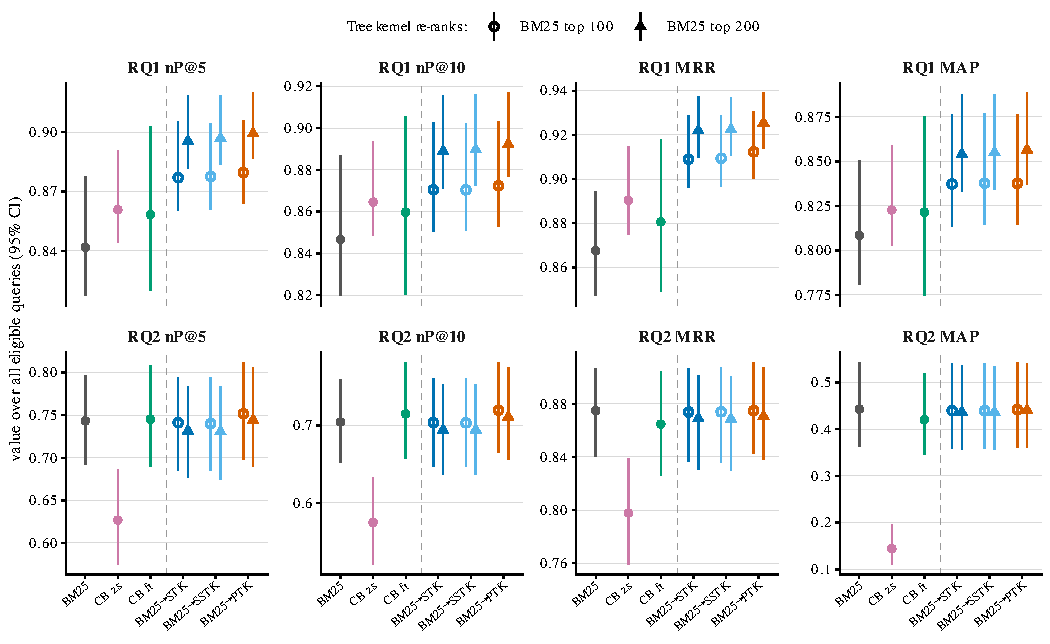
\includegraphics[width=\textwidth]{figures/hybrid_full}\caption{Hybrid on every eligible query: BM25, CodeBERT and BM25's top 100 or 200 re-ranked by each tree kernel; value and 95\% confidence interval (bootstrap over functionalities). Top: RQ1, mean over the five clone types; bottom: RQ2.}\label{fig:hybridfull}\end{figure*}
\begin{figure*}[t]\centering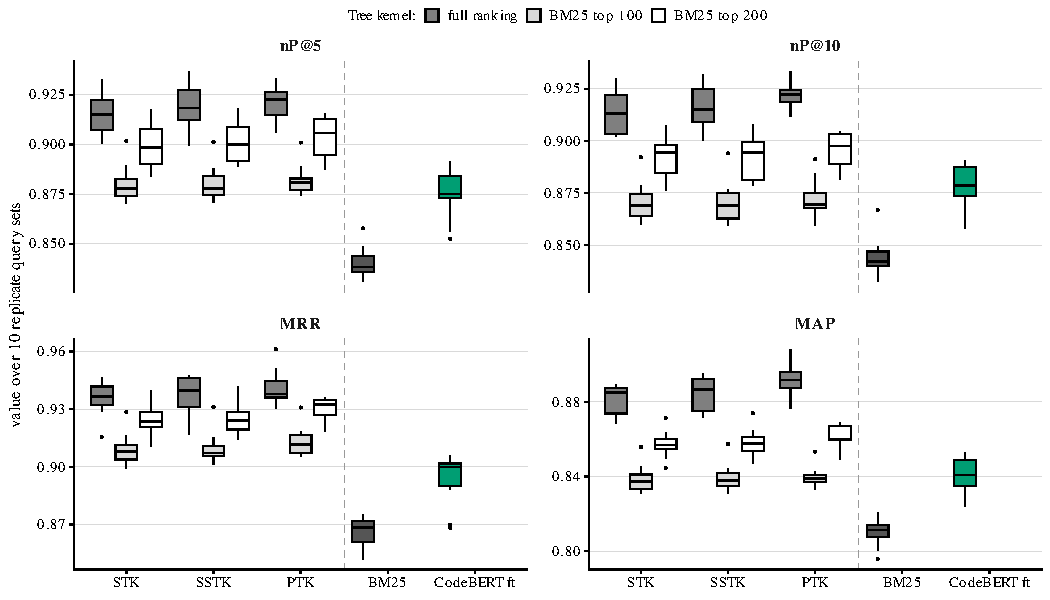
\includegraphics[width=\textwidth]{figures/hybrid_rq1}\caption{Hybrid against full ranking, RQ1 (mean over the five clone types), 10 replicate query sets: each tree kernel ranking the whole corpus or re-ranking BM25's top 100 or 200, next to BM25 and fine-tuned CodeBERT. \boxnote}\label{fig:hybrid1}\end{figure*}
\begin{figure*}[t]\centering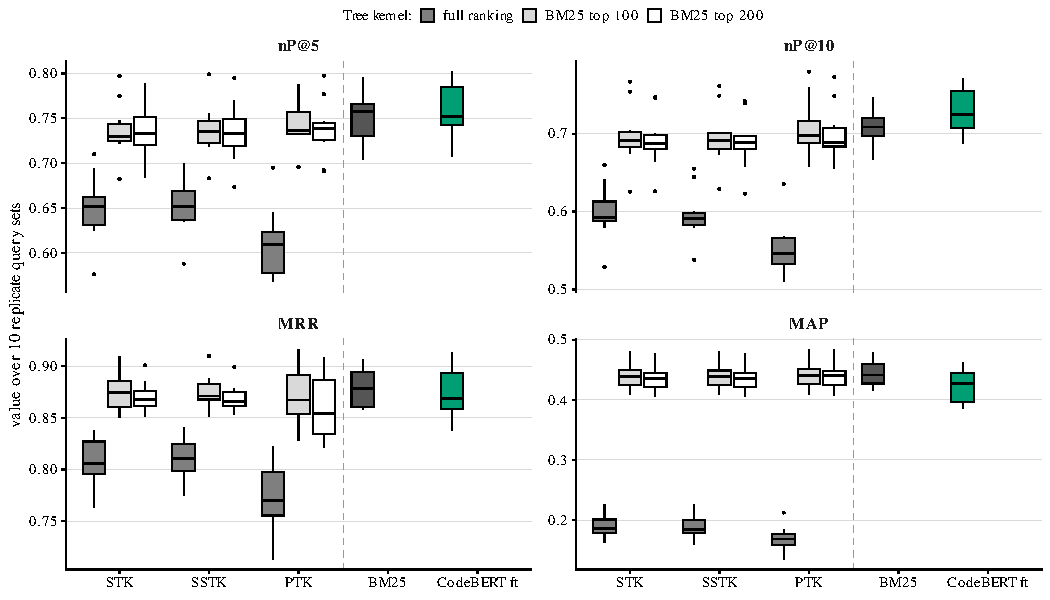
\includegraphics[width=\textwidth]{figures/hybrid_rq2}\caption{Hybrid against full ranking, RQ2 (functional similarity), 10 replicate query sets. \boxnote}\label{fig:hybrid2}\end{figure*}
\end{document}
